\chapter{Analiza Dziedziny}
\label{cha:anDziedziny}
%---------------------------------------------------------------------------

\section{Klasy i opis atrybutów}
\label{sec:klasyAtrybuty}
\begin{table}[H]
	\begin{tabular}{|l|l|l|} \hline
	\textbf{Klasa}	& \textbf{Atrybut} & \textbf{Opis} \\ \hline% \bottomrule
	Pojazd	& NumerRejestracyjny & Numer rejestracyjny pojazdu \\
	& Marka & Marka pojazdu \\
	& Model & Model pojazdu \\
	Samochód& & \\
	Motor& &  \\
	Autobus& & \\
	Parking	& IloscWolnychMiejsc & Określa ilość wolnych miejsc na parkingu \\
	MiejsceParkingowe	& Numer & Numer miejsca parkingowego \\
	& Typ & Typ miejsca parkingowego \\
	& Status & Określa status miejsca - wolne/zajęte \\
	Wjazd	& DataWjazdu & Data wjazdu na parking\\
	& CzasWjazdu & Czas wjazdu na parking \\
	& Pojazd & Określa pojazd, którego dotyczy wjazd \\
	Wyjazd	& DataWyjazdu & Data wyjazdu z parkingu\\
	& CzasWyjazdu & Czas wjazdu z parkingu \\
	& Pojazd & Określa pojazd, którego dotyczy wyjazd \\
	& StatusPlatnosci & Określa, czy płatność została zrealizowana \\
	Terminal & Status & Status określa możliwość wjazdu/wyjazdu na/z parkingu \\
	Szlaban & Status & Określa, czy szlaban jest otwarty/zamknięty\\
	Operator& Id & Id operatora \\
	& Imię & Imię operatora \\
	& Nazwisko & Nazwisko operatora \\
	BazaZdjęć& &  \\ \hline
	\end{tabular}
\end{table}


%---------------------------------------------------------------------------

\section{Diagramy klas  - relacje}
\label{sec:diagKlas}
% Diagram klas
\begin{figure}[H]
	\centering
	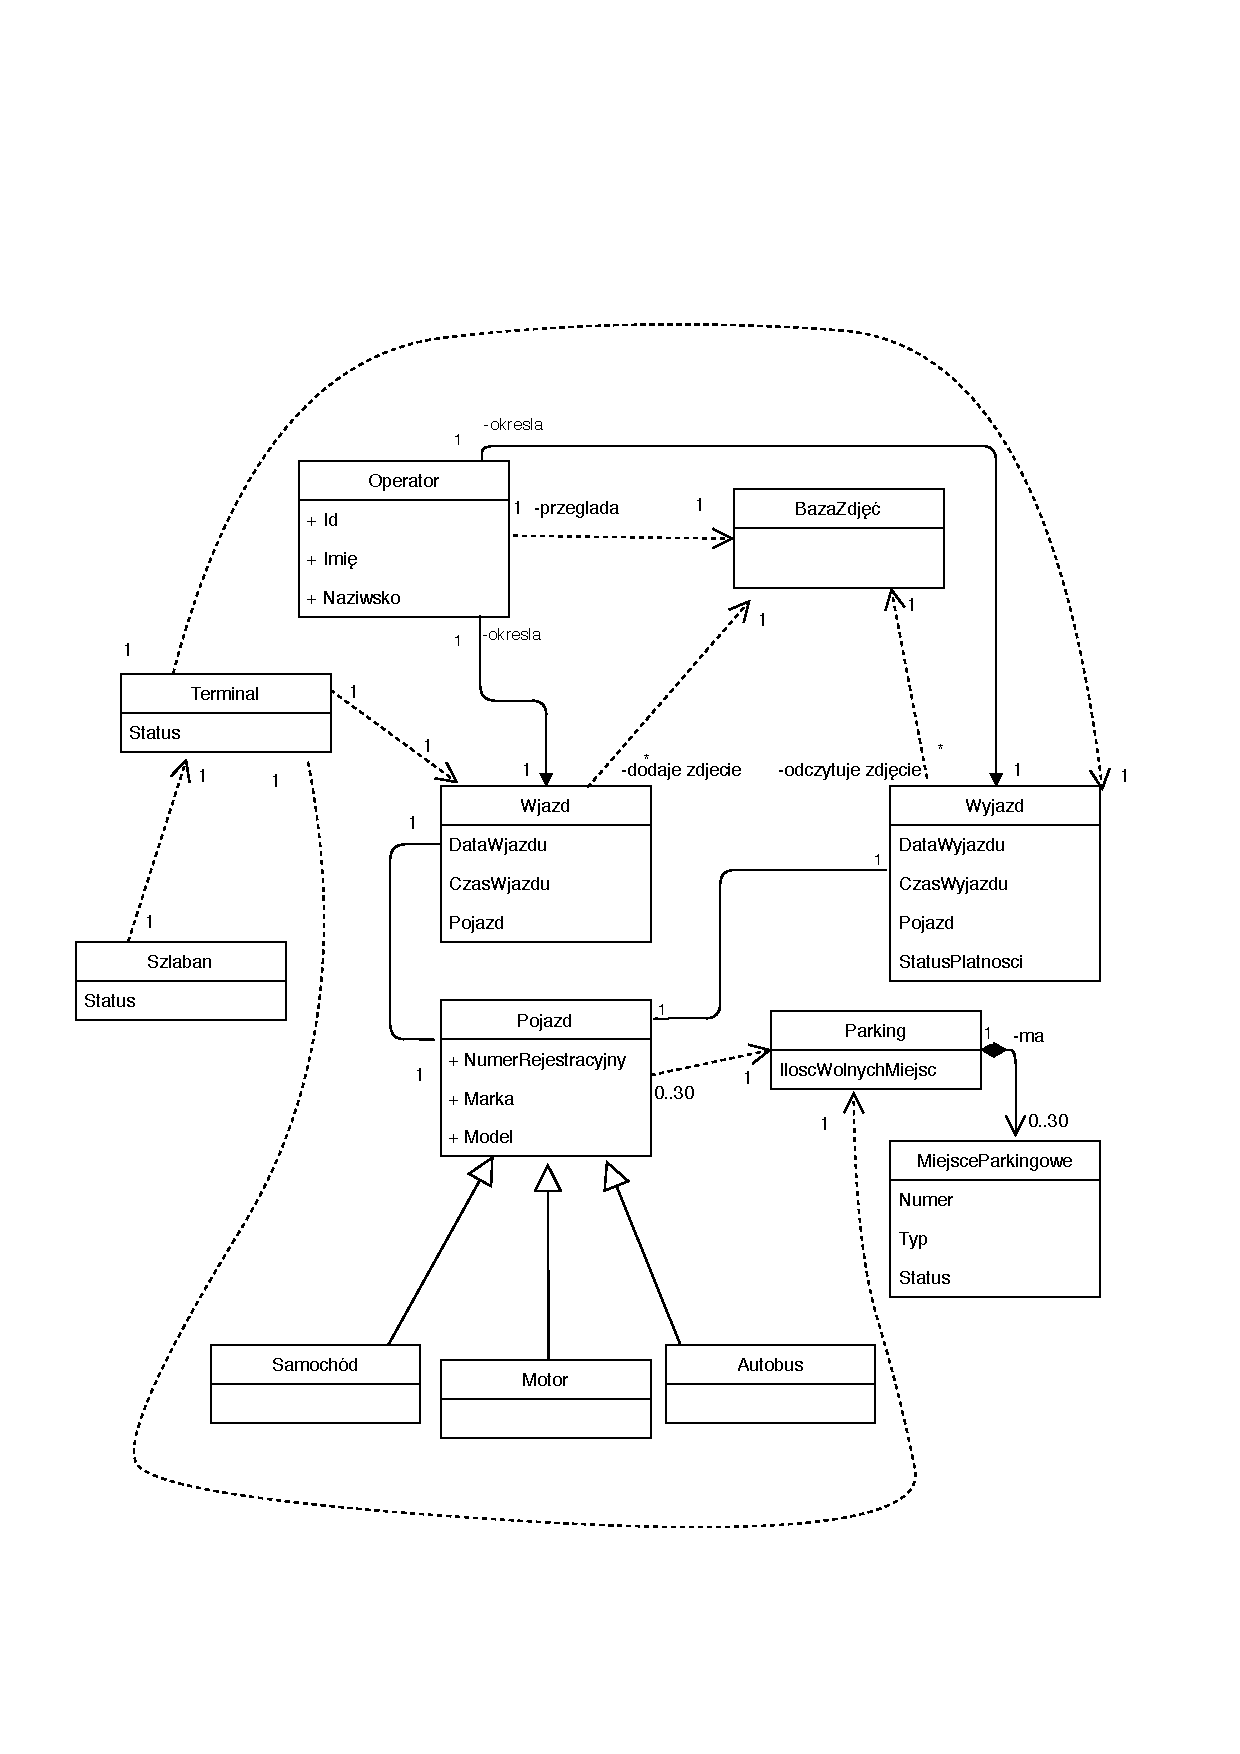
\includegraphics[width=150mm]{diagramy/DiagKlas.pdf}
	\caption{Diagram klas i relacje między nimi \label{overflow}}
\end{figure}


%---------------------------------------------------------------------------

\section{Diagramy stanów dla wybranych klas}
\label{sec:diagStanow}



%---------------------------------------------------------------------------

\section{Słownik pojęć}
\label{sec:slownik}

